\chapter{Introduction}

\section{Overview of neutron halo nuclei}
Over recent years, the study of neutron-rich nuclei has provided invaluable insights beyond the conventional nuclear models. A particularly intriguing subclass of neutron-rich nuclei is the \textit{neutron halo nuclei} \cite{Tanihata96}\cite{Tanihata13}, characterized by an extended halo of one or two loosely bound neutrons far from the core nucleus. The first discovery of a neutron halo nucleus was $^{11}$Li by I. Tanihata et al. \cite{Tanihata85}. As shown in Figure \ref{fig:Radius_11Li}, $^{11}$Li has a huge radius compared to the neighboring He, Li, Be and C isotopes with similar atomic mass numbers. Based on this discovery, I. Tanihata et al. proposed that $^{11}$Li has either a large deformation or a long tail in its matter distribution. Subsequently, P. G. Hansen and B. Jonson \cite{HansenandJonson} identified $^{11}$Li as a neutron halo nucleus, based on its large neutron radius relative to its $^{9}$Li core.

\begin{figure}
    \centering
    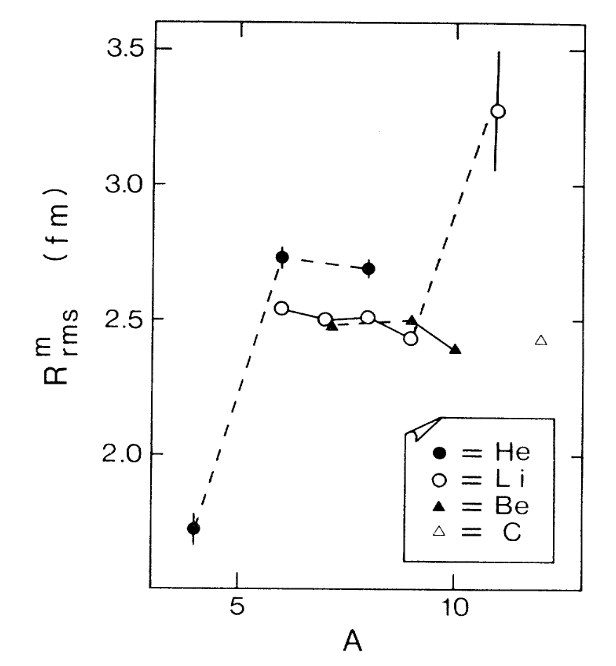
\includegraphics[width=6cm]{chapter1/Radius_of_11Li.png}
    \caption[Matter RMS radius of He, Li, Be and C isotopes]{Matter RMS radius of He, Li, Be and C isotopes. $^{11}$Li has a significantly larger radius than its neighbors He, Li, Be, and C \cite{Tanihata85}.}
    \label{fig:Radius_11Li}
\end{figure}

Further research on neutron halo nuclei has led to additional criteria for identifying them. One notable criterion is a small neutron separation energy. Compared to the separation energy of stable nuclei, typically around $S_n$ = 6 to 8 MeV, neutron halo nuclei have extremely small separation energies, less than 1 MeV. This leads to a large nuclear radius. This relationship between neutron separation energy and large radius can be understood from a simple example: Assume a core of nucleons which we model with a square-well potential given by 
\begin{align}
    V(r) =& \left\{ \begin{array}{ll}
                   -V_0 & (r \leq R) \\
                   0 & (r > R)
                   \end{array}  \right .
 \end{align}
A single neutron in the system will have a wavefunction outside of the potential given by 
\begin{align}
    \Psi(r) = \bigg(\frac{2\pi}{k}\bigg)\bigg(\frac{e^{-k r}}{r}\bigg)\bigg[\frac{e^{k R}}{(1+ k R)^{1/2}}\bigg], \label{eq:wavefunction}
\end{align}
where for simplification we consider only $l=0$. And the factor $k$ is given by 
\begin{align}
    &k = \sqrt{2\mu E/\hbar^2},
\end{align}
where $\mu$ is the effective mass of the system and $E$ is an eigenvalue of this wavefunction. In that case the neutron density distribution is given by
\begin{align}
    \rho(r) = |\Psi(r)|^2 \propto \frac{e^{-2k r}}{r^2}, \label{eq:neutron_density_distribution}
\end{align}
where the factor $k$ determines the tail of the distribution. When $k$ is small the distribution will have a long tail and vice versa. A long tail means that the nucleus has a large radius. We can then set $E = S_n$ to see that a small neutron separation energy gives a long tail and hence a large radius.

% halo feature 2
The narrow momentum distribution is also the criterion of halo nuclei. The momentum distribution of a neutron [$f (p)$] can be described by the Fourier transform of the eq. (\ref{eq:wavefunction}),
\begin{align}
    f(p) = \frac{C}{p^2+(\hbar k)^2},
\end{align}
where $p$ represents the momentum of the neutron and the width of the distribution is defined by $k$ which is related with the separation energy. This illustrates the Heisenberg's uncertainty principle: The smaller $k$, the wider density distribution, and the narrower momentum distribution. In Figure \ref{fig:Momentum_distribution}, the momentum distribution of $^{6}$H and $^{9}$Li are presented. $^{6}$H has a broad momentum distribution, with $\sigma = 77 \pm 5$ MeV/c, attributed to the non-halo structure of $^{8}$H. Conversely, $^{9}$Li has a significantly narrower momentum distribution, with a Gaussian peak at $\sigma  = 23 \pm 5$ MeV/c, which indicates $^{11}$Li is a halo nucleus.

\begin{figure}
    \centering
    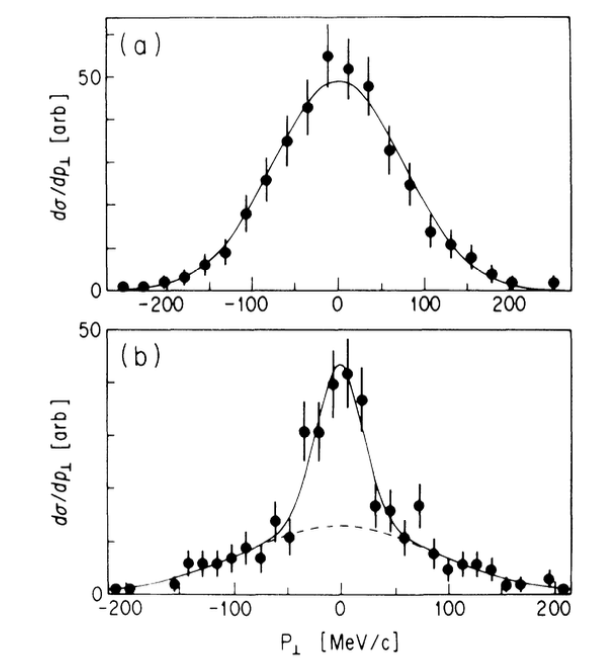
\includegraphics[width=7cm]{chapter1/Momentum_distribution.png}
    \caption[The momentum distribution of $^{6}$H and $^{9}$Li]{The momentum distribution of (a) $^{6}$H resulting from the $^{8}$H + C reaction, and (b) $^{9}$Li from $^{11}$Li + C reaction. Notably $^{9}$Li has extremely narrow momentum distribution, characterized by a narrow Gaussian peak with $\sigma  = 23 \pm 5$ MeV/c. \cite{Kobayashi88}}
    \label{fig:Momentum_distribution}
\end{figure}

% halo feature 3
Another critical criterion of halo nuclei is the orbital angular momentum of the valence neutron. The shape of the momentum distribution is influenced not only by the separation energy but also by the orbital angular momentum ($l$) due to the effect of the centrifugal barrier. The width of centrifugal barrier is proportional to $l(l+1)/r^2$, significantly affecting the neutron's density distribution. Riisager et al. \cite{Riisager} have performed calculations on the radius of a one-neutron halo system within a square-well potential, considering various separation energies and orbital angular momenta. In Figure \ref{fig:Angular_Orbital}, the $x$-axis represents the separation energy normalized by the size of the well potential $R_0$, while the $y$-axis signifies the root-mean-square (rms) radius, also normalized by $R_0$.  It is observed that the rms radius for $l$ = 0 or $l$ = 1 tends to increase significantly as the separation energy nears zero, suggestive of halo formation. However, for $l$ = 2, the rms radius remains close to $R_0$, indicating that it is challenging for nuclei with $l$ = 2 or higher to develop a halo structure.

\begin{figure}
    \centering
    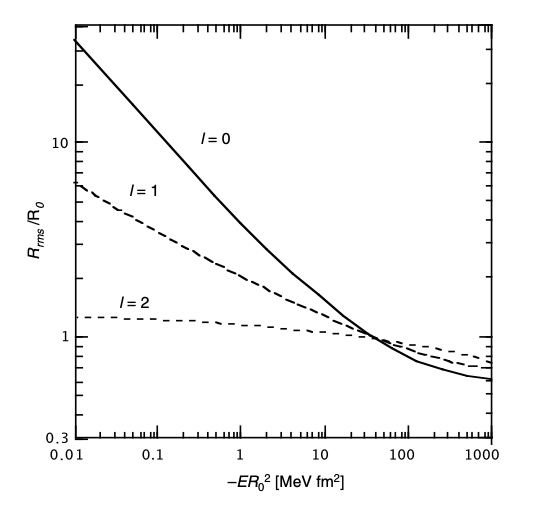
\includegraphics[width=8cm]{chapter1/Angular_Orbital.png}
    \caption{The rms radius of one-neutron halo for various separation energies and orbital angular momenta. \cite{Riisager}}
    \label{fig:Angular_Orbital}
\end{figure}

Through the consideration of halo nuclei criterion so far, we can understand the development mechanism of halo structures. A halo structure tends to be developed under conditions of low neutron separation energy, typically less than 1 MeV, and a low orbital angular momentum of $l$ = 0 or 1. With these conditions, the density distribution of the valence neutron(s) can extended to the outside of the core, leading to the formation of a halo structure.

% halo feature 4
Of all the criteria of halo nuclei, this work has a particular focus on the soft electric dipole ($E1$) mode, commonly referred to as soft $E1$ excitation. This phenomenon was predicted by P. G. Hansen and B. Jonson \cite{HansenandJonson}, as well as K. Ikeda et al.\cite{Ikeda}. Halo nuclei, comprised by a core and loosely bound valence neutron(s), can be polarized by an external electric field making the valence neutron(s) oscillate against the core nucleus. The soft $E1$ excitation mode between core and valence neutron(s) has a very low energy, typically less than 1 MeV, as the halo structure easily responds to the external electric field. Figure \ref{fig:E1_response} illustrates the $E1$ response of stable nuclei, neutron-skin nuclei and neutron halo nuclei. The $E1$ response appears in the photon absorption cross section $\sigma_\gamma$ and the  cross section is related to the reduced transition probability $B(E1)$ by eq. (\ref{eq:photon_absorption}). The giant dipole resonance (GDR) a high-energy dipole excitation mode around 15 - 20 MeV, arises from the oscillation between proton and neutron fluids. In neutron-skin nuclei, the pigmy dipole resonance (PDR) appears in mid-energy region ($\sim$ 10 MeV) due to the vibration between the neutron skin and core. The soft $E1$ excitation occurs in very low energy region, below 1 MeV, by the vibration between the core and loosely bounded valence neutron.
\begin{figure}
    \centering
    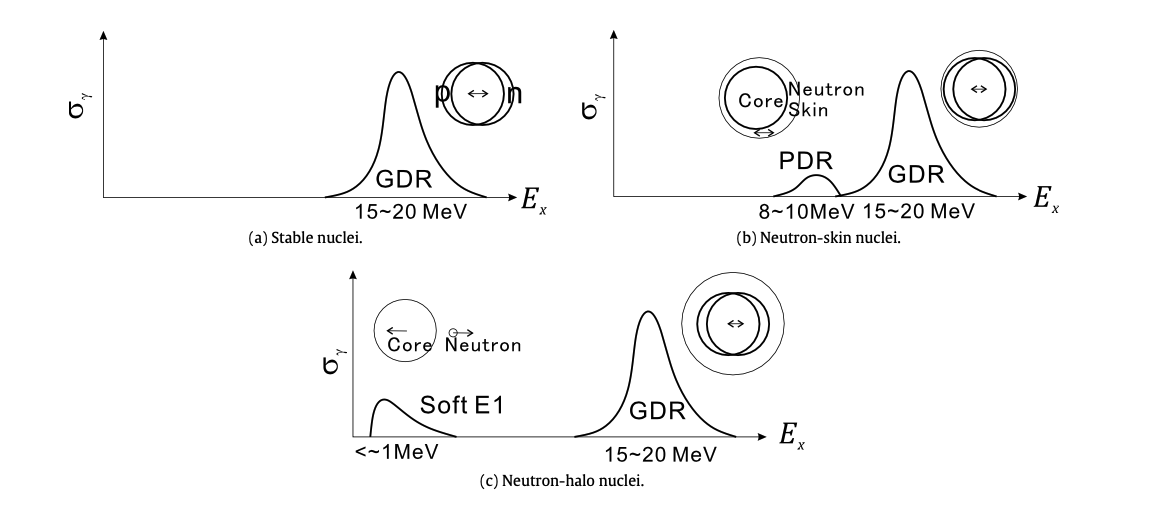
\includegraphics[width=\textwidth]{chapter1/E1_response.png}
    \caption{The schematic representation of $E1$ response of (a) stable nuclei, (b) neutron-skin nuclei and (c) neutron halo nuclei. \cite{Nakamura17}}
    \label{fig:E1_response}
\end{figure}

%BE1 explain
The strength of the dipole excitation mode is quantified by the $E1$ reduced transition probability $B(E1)$. The term 'reduced' in the context implies that the transition matrix element is independent of the magnetic sub-state of the initial and final states, according to the Wigner-Eckart theorem. The $E1$ reduced transition probability is defined as,
\begin{align}
    B(E1) = |\langle \Phi^f(\vec{r},\vec{q}) |e_{eff}^{E1}\hat{T}(E1)| \Phi^i(\vec{r})\rangle|^2 
\end{align}
where $e_{eff}^{E1}$ is effective charge $\hat{T}(E1) = rY_{1}(\Omega)$ represents the $E1$ transition operator, $\Phi_i(\vec{r})$ and $\Phi_f(\vec{r},\vec{q})$ are the initial and final states of the system respectively, which have the relative position vector between center of core and halo neutron $\vec{r}$ and the relative momentum $\vec{p} = \sqrt{2\mu E_{rel}}/\hbar$ as their component. To simplify, we assume the final state $\Phi_f$ as a plane wave as,
\begin{align}
    \Phi_f(\vec{r},\vec{q}) = \text{exp}(i\vec{r}\cdot\vec{q}).
\end{align}
Then, the $E1$ reduced transition probability for relative energy between core and halo neutron $E_{rel}$ can be rewritten as,
\begin{align}
    \frac{dB(E1)}{dE_x} &= |\langle \Phi^f(\vec{r},\vec{q}) ||e_{eff}^{\text{E1}}\hat{T}(E1)|| \Phi^i(\vec{r})\rangle|^2 \\
                        &= |\langle \text{exp}(i\vec{r}\cdot\vec{q}) ||e_{eff}^{\text{E1}}rY_{1}(\Omega)|| \Phi^i_{g.s.}\rangle|^2 \\
\end{align}
which is the form of Fourier transform of the ground state times $\vec{r}$ from $E1$ transition operator $\vec{r} \cdot \Phi_{g.s}(\vec{r})$. 
\textcolor{red}{and $J_i$ is the total angular momentum of the initial state.} \textcolor{blue}{Need a explanation of the meaning of B(E1)} To experimentally determine the E1 reduced transition probability, \textcolor{red}{it is necessary to excite the halo nucleus by photon absorption, achieved through Coulomb dissociation.} 

\begin{figure}
    \centering
    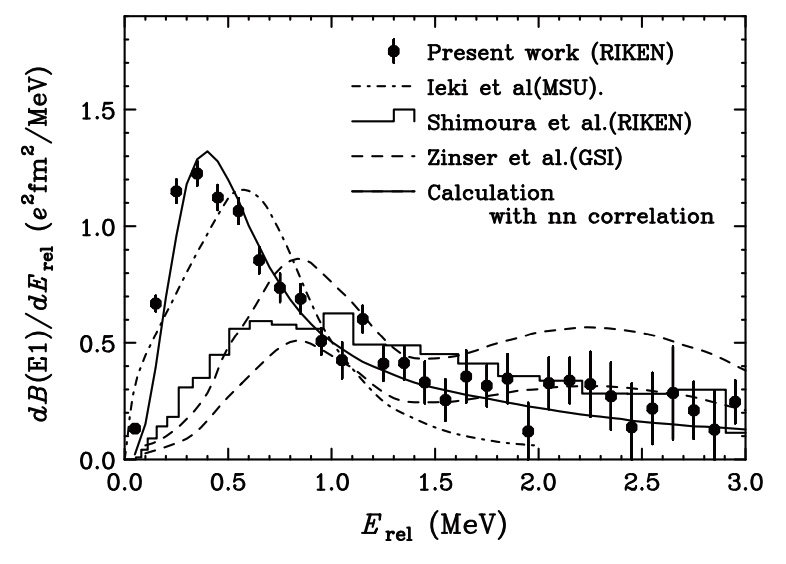
\includegraphics[width=8cm]{chapter1/B(E1)_11Li.png}
    \caption{B(E1) distribution of $^{11}$Li \cite{Nakamura06}}
    \label{fig:Coulomb_dissociation}
\end{figure}

The reason why we choose the E1 transition for investigating the neutron halo nuclei is that the E1 transition is the most dominant in middle energy region compared to other electromagnetic multi-polarity M1 or E2 \cite{Aumann}.

% The Coulomb dissociation cross section $\sigma_{CD}$ is directly related to the E1 reduced transition probability $dB(E1)$ and the photon number $N_{E1}(E1)$ as follows:
% \begin{align}
%     \frac{d\sigma_{CD}}{dE_x} \propto N_{E1}(E1) \frac{dB(E1)}{dE_x}.
% \end{align}
% Furthermore, geometrical information about halo nuclei can be extracted from E1 reduced transition probability. From the non-weighted cluster sum rule by Esbensen et al. \cite{Esbensen}, the total E1 reduced transition probability $B(E1)_{tot}$ can be expressed as a function of the core-neutron(s) radius $\langle R^2 \rangle$:
% \begin{align}
%     B(E1)_{tot} \sim \frac{3}{4\pi} \frac{Z e^2}{\hbar c} \langle R^2 \rangle.
% \end{align}
% This information is crucial for discovering dineutron correlation in two neutron halo, which is a strong spatial correlation between two neutrons in the surface of nucleus. The opening angle between two valence neutrons can be estimated by the core-neutrons radius $\sqrt{\langle r^2_{c-nn} \rangle}$ and the neutron-neutron distance $\sqrt{\langle r^2_{nn} \rangle}$ as follows\cite{Bertulani07}\cite{Hagino07}:

% In the three-body calculation, the dineutron correlation also can be estimated.
When we assume the orbital mixture of valance neutrons in $^{11}$Li, we can write the $^{11}$Li wavefunction as follows:
\begin{align}
    \Psi(^{11}\text{Li}) = \psi(^{9}\text{Li}) \otimes [\alpha |1p_{1/2} \rangle^2 + \beta |2s_{1/2} \rangle^2]
\end{align}

\begin{align}
    \langle \cos \theta_{nn} \rangle &= \langle \Psi({}^{11}\text{Li}) | \cos \theta_{nn} | \Psi({}^{11}\text{Li}) \rangle \notag \\
    &= \alpha^2 \langle (1d_{5/2})^2 | \cos \theta_{nn} | (1d_{5/2})^2 \rangle + \beta^2 \langle (2s_{1/2})^2 | \cos \theta_{nn} | (2s_{1/2})^2 \rangle \notag \\
    &\hspace{4mm} + 2\alpha \beta \langle (1d_{5/2})^2 | \cos \theta_{nn} | (2s_{1/2})^2 \rangle \notag \\
    &= 2\alpha \beta \langle (1d_{5/2})^2 | \cos \theta_{nn} | (2s_{1/2})^2 \rangle
\end{align}

where $|(1d_{5/2}^2)$ represents $|\psi({}^{15}\text{B})\otimes|$


\begin{figure}
    \centering
    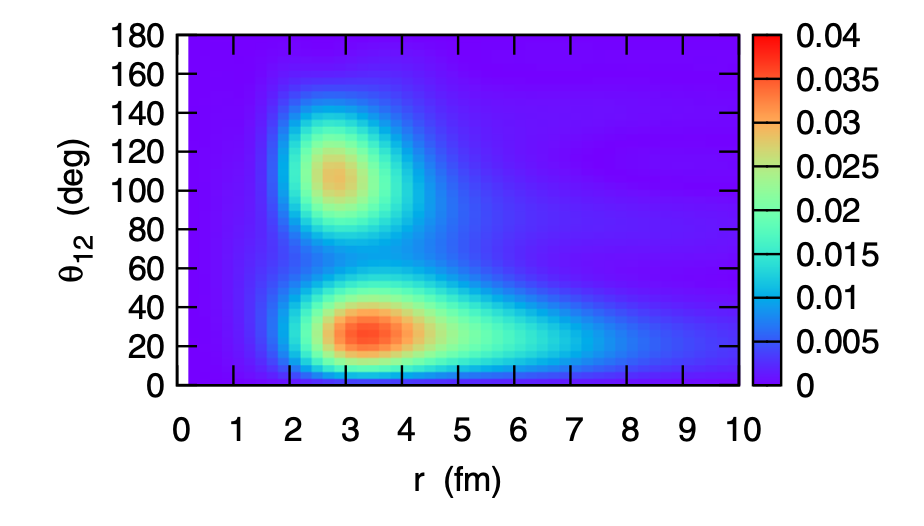
\includegraphics[width=8cm]{chapter1/11Li_Dineutron.png}
    \caption{The dineutron correlation in $^{11}$Li. \cite{Hagino05}}
    \label{fig:dineutron}
\end{figure}


\section{The halo structure of ${}^{17}$B}
There are two two-neutron halo nuclei in boron isotopes, $^{17}$B and $^{19}$B. Both nuclei are considered as a two neutron halo nuclei because of the small two neutron separation energy and large radius. \cite{Suzuki99}

Recently, in boron isotopes, the reduced E1 transition probability of $^{19}$B is observed by K. J. Cook et al.\cite{KJCook} using Coulomb dissociation method. $^{19}$B has been considered as a two neutron halo nuclei, but on the other hand, also considered as 4 neutron halo nucleus or neutron skin nucleus. $^{19}$B has very small two neutron separation energy, $S_{2n} = 0.088(564)$ MeV \cite{Wang19B}, but also its core $^{17}$B has small 2n separation energy, $S_{2n} = 1.384(205)$ MeV and large radius\cite{Suzuki99}. And also the valance neutrons of $^{19}$ are occupied in sd-shell, which makes the orbital mixing of $1d_{5/2}$ and $2s_{1/2}$. If 4 neutrons occupy the $1d_{5/2}$ orbital, because of the high centrifugal barrier, halo structure cannot develope. On the other hand, if 2 neutrons occupy the $2s_{1/2}$ orbital, the halo structure can be developed. The result of K. J. Cook et al. extracted the reduced E1 transition probability of $^{19}$B and the peak was observed around 0.5 MeV. This result shows that the $^{19}$B has very strong soft E1 mode, which means that the halo structure of $^{19}$B is developed. Also, a dineutron correlation is calculated in $^{19}$B case \cite{Hagino05}, and the result shows that the dineutron correlation is strongly developed in $^{19}$B. In figure \ref{dineutron} the opening angle of two neutron of $^{19}$B is shown. 


\begin{figure}[t]
    \centering
    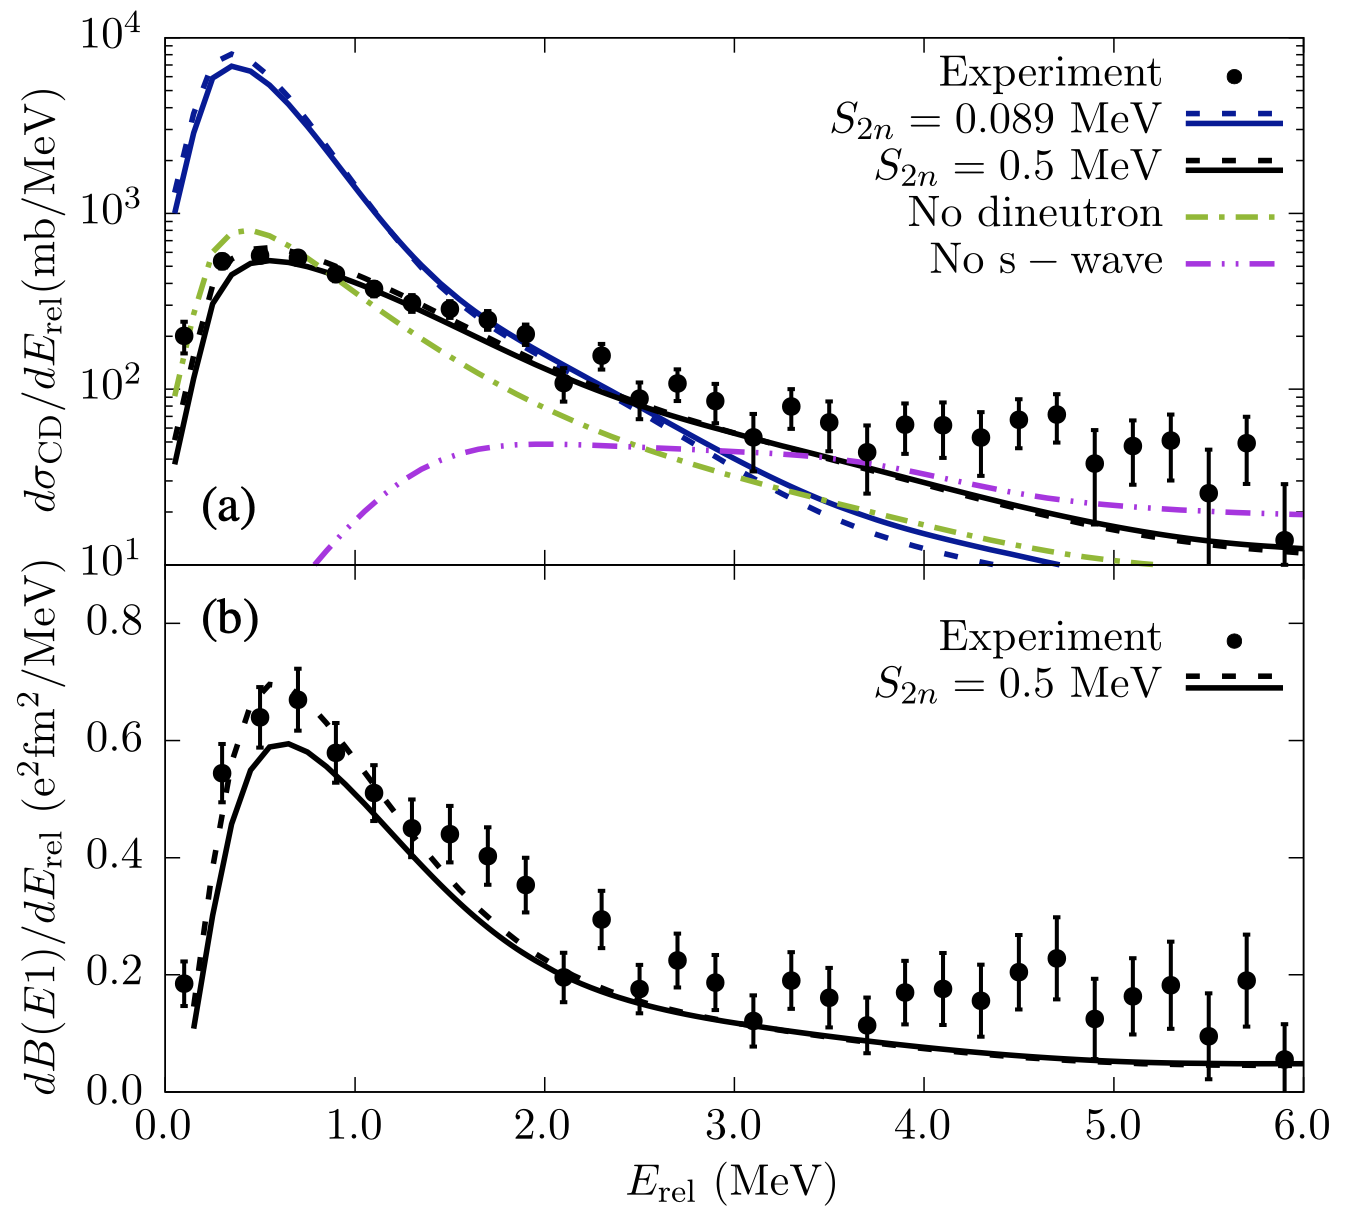
\includegraphics[width=10cm]{chapter1/19B_B(E1).png}
    \caption[The B(E1) distribution of $^{19}$B]{The B(E1) distribution of $^{19}$B. The peak at 0.5 MeV is the soft E1 excitation.}
\end{figure}


\begin{figure}[t]
    \centering
    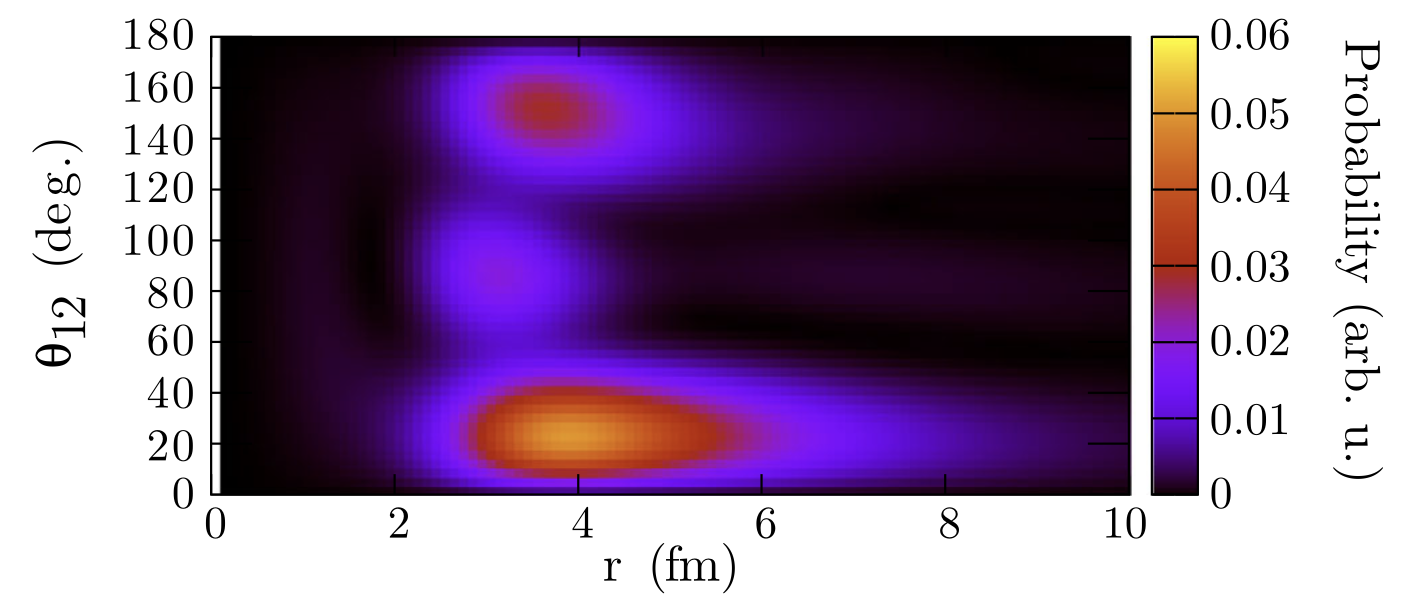
\includegraphics[width=10cm]{chapter1/19B_Dineutron.png}
    \caption{The opening angle distribution of two valance neutrons of $^{19}$B.}
    \label{dineutron}
\end{figure}


After revealing the structure of $^{19}$B, the structure of $^{17}$B got attention. The first discover of $^{17}$B as a halo nucleus was by T. Suzuki.\cite{Suzuki99} $^{17}$B has small 2n separation energy, and large radius. And also, the valance neutrons of $^{17}$B are occupied in sd-shell, which makes the orbital mixing of $1d_{5/2}$ and $2s_{1/2}$ as same as $^{19}$B. According to the angular orbital momentum dependency, the halo structure can be developed when the two valance neutron occupy $2s_{1/2}$ orbital. 

\begin{align}
    \Psi(^{17}\text{B}) = \psi(^{15}\text{B}) \otimes [\alpha |1d_{5/2} \rangle^2 + \beta |2s_{1/2} \rangle^2]
\end{align}

But recently, Z. H. Yang et al. \cite{ZHYang} shows a strong evidence that $^{17}$B might not be a two neutron halo nuclei. He performed the quasi-free ($p,pn$) scattering reaction and extracted the relative energy distribution of $^{16}$B. He assumed that the knocked-out neutron from the $^{17}$B  should almost come from $1d_{5/2}$ or $2s_{1/2}$ orbital and got the relative energy distribution of $^{16}$B. (Figure \ref{fig:quasi-free}) And also, he obtained the spectroscopic factors for $1d_{5/2}$ and $2s_{1/2}$ orbital and there was surprisingly small percentage 9(2)\% of $2s_{1/2}$ orbital. This result is very different from the ones, which are 36(19)\%, 69(20)\%, 50(10)\% and by T. Suzuki and Y. Yamaguchi. \cite{Suzuki99} \cite{Suzuki02} \cite{Yamaguchi} Also A. Estradé et al. \cite{Estrade} shows proton radii of boron isotope. In this research, $^{17}$B has very thick neuron surface, 0.51(11) fm, which might indicates a neutron skin structure. 

\begin{figure}
    \centering
    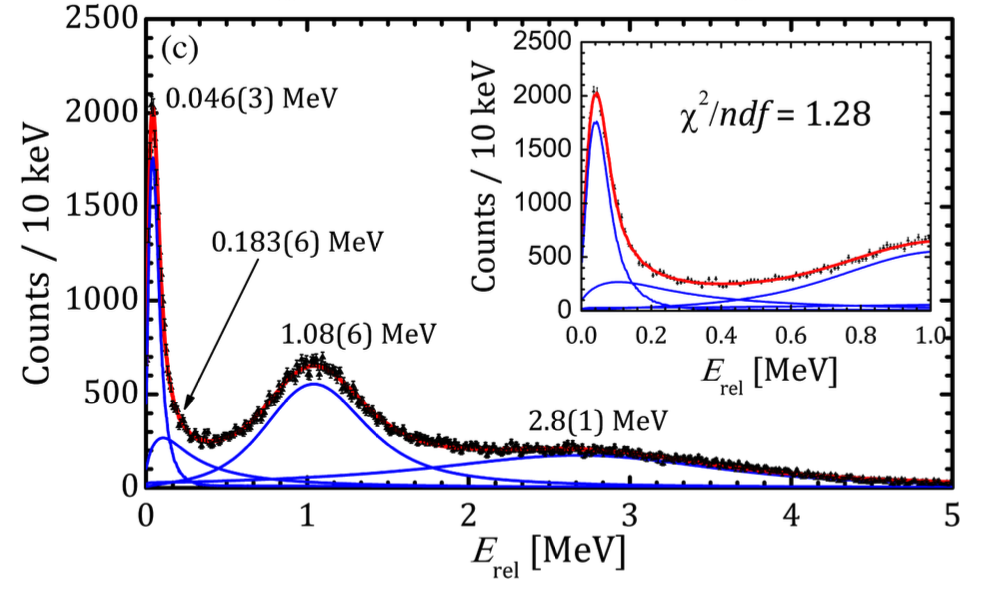
\includegraphics[width=10cm]{chapter1/17B_ZHYang.png}
    \caption{The relative energy distribution of $^{16}$B.\cite{ZHYang}}
    \label{fig:quasi-free}
\end{figure}

\begin{figure}
    \centering
    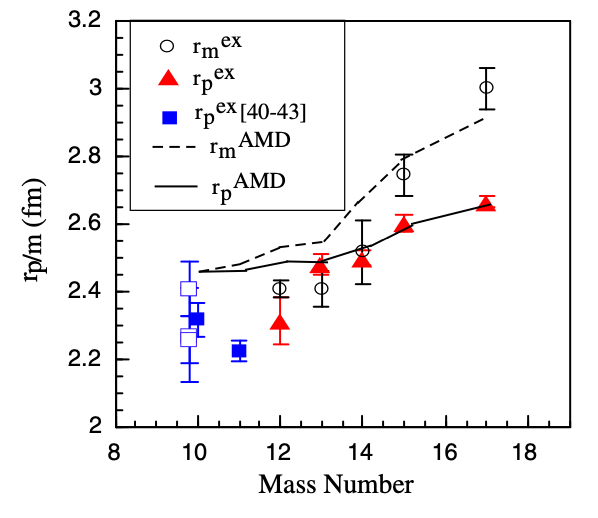
\includegraphics[width=8cm]{chapter1/RadiiofBoron.png}
    \caption{The proton radii ($r_p$) and rms matter radii ($r_m$) of $^{12-17}$B. \cite{Estrade}}
\end{figure}
So, in this research, we study the Soft E1 excitation of $^{17}$B for the first, which can be the final key for deciding halo strength of $^{17}$B. In this thesis, we will discuss the Coulomb Dissociation of $^{17}$B as a tool for searching the Soft E1 excitation of $^{17}$B. 


